\chapter{Thực nghiệm và Đánh giá}
\label{chap:thuc_nghiem_danh_gia}

Chương này trình bày các thực nghiệm được thực hiện để đánh giá hiệu suất của PhaBERT trong bài toán phân loại hệ gen thực khuẩn thể. Quy trình xây dựng tập dữ liệu, kiến trúc mô hình và chiến lược huấn luyện đã được mô tả chi tiết trong Chương~\ref{chap:method}, chương này tập trung vào đánh giá thực nghiệm, so sánh với các phương pháp tiên tiến, và phân tích hiệu quả của phương pháp đề xuất. Nội dung được tổ chức như sau: thiết lập thực nghiệm và môi trường tính toán, kết quả so sánh trên bốn nhóm độ dài contig, thảo luận về các yếu tố đóng góp vào hiệu suất cùng ý nghĩa thực tiễn của cải thiện, và kết luận chương.

\section{Thiết lập thực nghiệm}
\label{sec:thiet_lap_thuc_nghiem}

Tập dữ liệu được xây dựng theo quy trình mô tả trong Phần~\ref{sec:data_preprocessing}, bao gồm 2.241 hệ gen thực khuẩn thể hoàn chỉnh (707 ôn hòa và 1.534 độc lực), được chia thành bốn nhóm theo độ dài contig: A (100--400 bp), B (400--800 bp), C (800--1.200 bp) và D (1.200--1.800 bp). Việc phân chia thành bốn nhóm độ dài theo DeePhage~\cite{wu2021deephage} cho phép đánh giá một cách có hệ thống ảnh hưởng của độ dài contig đến hiệu suất phân loại, một yếu tố đặc biệt quan trọng trong phân tích dữ liệu hệ gen môi trường, nơi các contig thu được sau quá trình lắp ráp thường có độ dài biến thiên lớn~\cite{ghurye2016metagenomic}. Các contig được tạo bằng phương pháp cửa sổ trượt với bộ tham số riêng cho từng nhóm (Bảng~\ref{tab:sliding_window_params}), sau đó được tăng cường bằng chuỗi bổ sung đảo ngược và cân bằng lớp bằng phương pháp lấy mẫu giảm ngẫu nhiên trên tập huấn luyện (Bảng~\ref{tab:dataset_statistics}). Quá trình đánh giá được thực hiện theo phương pháp kiểm định chéo phân tầng 5 phần với tỷ lệ huấn luyện:kiểm định là 8:2 trong mỗi phần, nhằm đảm bảo phân bố lớp nhất quán giữa các tập con~\cite{wu2021deephage}.

PhaBERT được so sánh với bốn phương pháp đại diện cho các hướng tiếp cận khác nhau trong bài toán phân loại hệ gen thực khuẩn thể: (1)~DNABERT-2~\cite{zhou2023dnabert} với đầu phân loại tuyến tính đơn giản, đóng vai trò đường cơ sở trực tiếp để đánh giá đóng góp riêng của kiến trúc MKC; (2)~DeePhage~\cite{wu2021deephage}, phương pháp học sâu sử dụng mạng nơ-ron tích chập trên mã hóa one-hot mà không qua giai đoạn tiền huấn luyện; (3)~PhaTYP~\cite{shang2023phatyp}, phương pháp dựa trên BERT với đặc trưng protein được hỗ trợ bởi Prodigal~\cite{hyatt2010prodigal}; và (4)~ProkBERT~\cite{ligeti2024prokbert}, mô hình BERT tiền huấn luyện trên hệ gen sinh vật nhân sơ với phương pháp mã hóa LCA k-mer chồng lấn. DeepPL~\cite{zhang2024deeppl} không được đưa vào so sánh do mô hình DNABERT nền tảng của phương pháp này sử dụng embedding vị trí học được với giới hạn tối đa 512 bp, không phù hợp cho việc đánh giá trên các contig có độ dài lên đến 1.800 bp trong thiết kế thực nghiệm này. Bốn phương pháp được lựa chọn đại diện cho các chiến lược biểu diễn chuỗi khác nhau: mã hóa BPE (DNABERT-2 và PhaBERT), mã hóa dựa trên protein (PhaTYP), mã hóa one-hot (DeePhage) và mã hóa k-mer (ProkBERT), cho phép đánh giá toàn diện ảnh hưởng của chiến lược biểu diễn đầu vào đến hiệu suất phân loại.

Hiệu suất phân loại được đánh giá bằng ba chỉ số, nhất quán với các nghiên cứu trước~\cite{wu2021deephage,shang2023phatyp}: độ nhạy (\textit{sensitivity}, $\text{Sn} = \text{TP}/(\text{TP}+\text{FN})$) đo khả năng phát hiện đúng thực khuẩn thể độc lực, độ đặc hiệu (\textit{specificity}, $\text{Sp} = \text{TN}/(\text{TN}+\text{FP})$) đo khả năng nhận diện đúng thực khuẩn thể ôn hòa, và độ chính xác tổng thể (\textit{accuracy}, $\text{Acc} = (\text{TP}+\text{TN})/(\text{TP}+\text{FN}+\text{TN}+\text{FP})$) đo hiệu suất phân loại trên toàn bộ tập dữ liệu.

\section{Tài nguyên tính toán}
\label{sec:tai_nguyen_tinh_toan}

Tất cả các thực nghiệm được thực hiện trên môi trường phần cứng bao gồm GPU NVIDIA RTX 5070Ti, CPU Intel i5 13500, và 64GB RAM. Môi trường phần mềm sử dụng Python 3.10 làm ngôn ngữ lập trình chính, kết hợp với PyTorch 2.1.0 và CUDA 12.1 cho việc huấn luyện mô hình học sâu trên GPU. Thư viện Transformers phiên bản 4.28.0 từ Hugging Face được sử dụng để tải và tinh chỉnh mô hình DNABERT-2 tiền huấn luyện. Ngoài ra, các thư viện hỗ trợ bao gồm NumPy 1.26.4 cho xử lý mảng số, Pandas 2.2.3 cho thao tác dữ liệu dạng bảng, Scikit-learn 1.6.1 cho các phương pháp học máy baseline và đánh giá mô hình, BioPython 1.85 cho xử lý chuỗi sinh học, và Matplotlib 3.9.4 cùng Seaborn 0.13.2 cho trực quan hóa kết quả.

\section{Kết quả thực nghiệm}
\label{sec:ket_qua}

\subsection{Đánh giá đóng góp của MKC}

Để đánh giá đóng góp của kiến trúc chuyên biệt cho tác vụ, học viên thực hiện nghiên cứu loại bỏ thành phần nhằm so sánh bảy cấu hình: (1)~đường cơ sở DNABERT-2, tức mô hình DNABERT-2 chỉ với đầu phân loại tuyến tính đơn giản, không tích hợp mô-đun MKC; (2)~PhaBERT, kiến trúc đề xuất đầy đủ với nhánh CNN đa cửa sổ kết hợp gộp trung bình có mặt nạ toàn cục; (3)~DNABERT-2-CNN, biến thể chỉ sử dụng nhánh CNN đa cửa sổ mà không có nhánh gộp toàn cục; (4)~DNABERT-2-P, biến thể thay thế toàn bộ mô-đun MKC bằng cơ chế gộp chú ý; (5)~PhaBERT-NO-K5, biến thể loại bỏ nhánh tích chập kích thước cửa sổ 5; (6)~PhaBERT-NO-K3, biến thể loại bỏ nhánh tích chập kích thước cửa sổ 3; và (7)~PhaBERT-NO-K7, biến thể loại bỏ nhánh tích chập kích thước cửa sổ 7. So sánh đường cơ sở DNABERT-2 với PhaBERT cho phép đánh giá đóng góp tổng thể của mô-đun MKC, so sánh DNABERT-2-CNN và DNABERT-2-P với đường cơ sở cho phép tách biệt đóng góp riêng của từng thành phần, trong khi ba biến thể PhaBERT-NO-K cho phép đánh giá đóng góp riêng của từng kích thước cửa sổ tích chập trong nhánh CNN đa cửa sổ. Bảng~\ref{tab:ablation_results} trình bày kết quả so sánh chi tiết.

\begin{table}[h]
    \centering
    \caption{Nghiên cứu loại bỏ thành phần: so sánh các cấu hình trên bốn nhóm độ dài contig}
    \label{tab:ablation_results}
    \resizebox{\textwidth}{!}{%
    \begin{tabular}{rclllll}
        \hline
        Cấu hình & Chỉ số (\%) &
        \multicolumn{1}{c}{\begin{tabular}[c]{@{}c@{}}Nhóm A\\ (100--400 bp)\end{tabular}} &
        \multicolumn{1}{c}{\begin{tabular}[c]{@{}c@{}}Nhóm B\\ (400--800 bp)\end{tabular}} &
        \multicolumn{1}{c}{\begin{tabular}[c]{@{}c@{}}Nhóm C\\ (800--1.200 bp)\end{tabular}} &
        \multicolumn{1}{c}{\begin{tabular}[c]{@{}c@{}}Nhóm D\\ (1.200--1.800 bp)\end{tabular}} \\ \hline
        \multirow{3}{*}{DNABERT-2}       & Sn  & 83,68 & 87,24 & 87,68 & 88,75 \\
                                         & Sp  & 73,25 & 79,27 & 85,75 & 86,99 \\
                                         & Acc & 81,52 & 85,56 & 87,25 & 88,36 \\ \hline
        \multirow{3}{*}{PhaBERT}         & Sn  & 82,07 & 88,11 & 90,69 & \textbf{92,38} \\
                                         & Sp  & \textbf{81,86} & 84,53 & \textbf{86,92} & 87,63 \\
                                         & Acc & 82,01 & 87,33 & 89,90 & \textbf{91,38} \\ \hline
        \multirow{3}{*}{DNABERT-2-CNN}   & Sn  & 82,68 & 88,11 & \textbf{91,21} & 91,75 \\
                                         & Sp  & 80,44 & \textbf{84,63} & 86,25 & 88,58 \\
                                         & Acc & 82,18 & 87,36 & \textbf{90,16} & 91,07 \\ \hline
        \multirow{3}{*}{DNABERT-2-P}    & Sn  & \textbf{85,12} & \textbf{89,04} & 90,84 & 91,72 \\
                                         & Sp  & 77,65 & 84,49 & 86,30 & \textbf{88,74} \\
                                         & Acc & \textbf{83,54} & \textbf{87,63} & 89,88 & 91,08 \\ \hline
        \multirow{3}{*}{PhaBERT-NO-K5}   & Sn  & 85,05 & 88,31 & 91,12 & 92,22 \\
                                         & Sp  & 78,03 & 84,19 & 86,71 & 86,92 \\
                                         & Acc & 83,56 & 87,44 & 90,18 & 90,99 \\ \hline
        \multirow{3}{*}{PhaBERT-NO-K3}   & Sn  & 84,18 & 88,61 & 91,80 & 92,22 \\
                                         & Sp  & 78,65 & 83,50 & 85,53 & 86,92 \\
                                         & Acc & 83,00 & 85,51 & 90,49 & 91,05 \\ \hline
        \multirow{3}{*}{PhaBERT-NO-K7}   & Sn  & 83,62 & 89,54 & 90,95 & 91,56 \\
                                         & Sp  & 78,47 & 82,06 & 87,47 & 89,20 \\
                                         & Acc & 82,55 & 87,95 & 90,21 & 91,05 \\ \hline
    \end{tabular}%
    }
\end{table}

Cả ba biến thể (PhaBERT, DNABERT-2-CNN, DNABERT-2-P) đều vượt trội so với đường cơ sở DNABERT-2 một cách nhất quán trên tất cả các nhóm độ dài, xác nhận rằng các thành phần kiến trúc bổ sung mang lại cải thiện có ý nghĩa so với việc chỉ sử dụng đầu phân loại tuyến tính. So với đường cơ sở DNABERT-2, PhaBERT cải thiện độ chính xác lần lượt 0,49\% (Nhóm A), 1,77\% (Nhóm B), 2,65\% (Nhóm C) và 3,02\% (Nhóm D), với mức cải thiện tăng dần theo độ dài contig. Đặc biệt, độ đặc hiệu được cải thiện đáng kể: tăng 8,61\% ở Nhóm A (từ 73,25\% lên 81,86\%) và 5,26\% ở Nhóm B (từ 79,27\% lên 84,53\%), cho thấy mô-đun MKC nâng cao đáng kể khả năng nhận diện thực khuẩn thể ôn hòa. Xu hướng cải thiện tăng dần theo độ dài phản ánh đặc tính của nhánh CNN đa cửa sổ với ba kích thước bộ lọc (3, 5, 7) theo thiết kế kế thừa từ TextCNN~\cite{kim2014convolutional}: khi chuỗi dài hơn, các mô-típ chức năng đặc trưng của hệ gen thực khuẩn thể trở nên hoàn chỉnh và phong phú hơn, cho phép các bộ lọc tích chập ở nhiều tỷ lệ không gian khai thác hiệu quả hơn các mẫu cục bộ.

So sánh hai thành phần riêng lẻ cho thấy sự khác biệt đáng chú ý giữa DNABERT-2-CNN (chỉ nhánh CNN đa cửa sổ) và DNABERT-2-P (chỉ gộp chú ý). DNABERT-2-P đạt độ chính xác cao hơn ở Nhóm A (83,54\% so với 82,18\%) và Nhóm B (87,63\% so với 87,36\%), trong khi DNABERT-2-CNN nhỉnh hơn ở Nhóm C (90,16\% so với 89,88\%) và hai biến thể đạt kết quả gần tương đương ở Nhóm D (91,07\% so với 91,08\%). Xu hướng này cho thấy gộp chú ý mang lại lợi thế trên các contig ngắn, nơi việc tập trung vào các vùng có tính thông tin cao giúp bù đắp cho lượng thông tin trình tự hạn chế, trong khi CNN đa cửa sổ phát huy hiệu quả hơn trên các contig dài nhờ khả năng khai thác các mô-típ chức năng hoàn chỉnh hơn.

PhaBERT, kết hợp cả hai nhánh CNN đa cửa sổ và gộp trung bình có mặt nạ, thể hiện ưu thế rõ rệt trên contig dài: đạt độ chính xác cao nhất ở Nhóm D (91,38\%) cùng độ nhạy vượt trội (92,38\% so với 91,75\% của DNABERT-2-CNN và 91,72\% của DNABERT-2-P). Đồng thời, PhaBERT đạt độ đặc hiệu cao nhất trong các cấu hình ablation ở Nhóm A (81,86\%) và Nhóm C (86,92\%), cho thấy sự kết hợp hai nhánh cải thiện khả năng nhận diện thực khuẩn thể ôn hòa. Nhìn tổng thể, việc kết hợp trích xuất đặc trưng cục bộ đa tỷ lệ từ CNN với tổng hợp thông tin toàn cục từ gộp trung bình có mặt nạ mang lại hiệu suất cân bằng và ổn định hơn so với từng thành phần riêng lẻ trên toàn phổ độ dài contig.

Kết quả loại bỏ từng kích thước cửa sổ tích chập (PhaBERT-NO-K5, PhaBERT-NO-K3, PhaBERT-NO-K7) cho thấy mỗi nhánh tích chập đóng góp thực sự so với đường cơ sở DNABERT-2, nhưng thông tin giữa các nhánh chồng lấn đáng kể. Cụ thể, loại bỏ bất kỳ một kích thước cửa sổ nào chỉ làm thay đổi độ chính xác trong khoảng $\pm$0,3--1,5\% so với mô hình đầy đủ, nằm trong biên dao động của kiểm định chéo 5 phần. Trên contig ngắn (Nhóm A), các biến thể thiếu một nhánh thậm chí đạt độ chính xác cao hơn mô hình đầy đủ (83,56\% của PhaBERT-NO-K5 so với 82,01\% của PhaBERT), phản ánh hiệu ứng chính quy hóa: khi tín hiệu trình tự hạn chế, ít tham số hơn giúp mô hình tổng quát hóa tốt hơn do giảm nguy cơ quá khớp. Ngược lại, trên contig dài nhất (Nhóm D), mô hình đầy đủ đạt kết quả cao nhất (91,38\% so với 90,99--91,05\% của các biến thể NO-K), cho thấy lợi ích của việc khai thác đặc trưng đa tỷ lệ chỉ phát huy rõ ràng khi trình tự đủ dài để chứa các mô-típ chức năng đa dạng ở nhiều kích thước khác nhau.

Điểm đáng chú ý là so sánh giữa DNABERT-2-CNN (ba nhánh CNN, không có gộp toàn cục, 384 chiều đặc trưng) với các biến thể PhaBERT-NO-K (hai nhánh CNN kết hợp gộp trung bình có mặt nạ, cũng 384 chiều đặc trưng): hai nhóm cấu hình này đạt hiệu suất gần tương đương trên hầu hết các nhóm. Kết quả này cho thấy việc thay thế một nhánh tích chập bằng nhánh gộp trung bình có mặt nạ mang lại hiệu quả tương đương, xác nhận rằng cả hai loại nhánh đều trích xuất thông tin phân loại ở mức tương đương từ biểu diễn ẩn của DNABERT-2. Nói cách khác, giá trị của kiến trúc MKC nằm ở việc cung cấp nhiều góc nhìn vào cùng một tín hiệu hệ gen, tạo biểu diễn ổn định hơn so với đường cơ sở---nhưng lợi ích biên giảm dần khi thêm nhiều nhánh, do thông tin giữa các nhánh chồng lấn đáng kể.

\subsection{So sánh với các phương pháp tiên tiến}

Bảng~\ref{tab:main_results} trình bày kết quả so sánh toàn diện giữa PhaBERT và các phương pháp tiên tiến trên bốn nhóm độ dài contig, sử dụng phương pháp kiểm định chéo phân tầng 5 phần.

\begin{table}[h]
    \centering
    \caption{So sánh hiệu suất PhaBERT, PhaTYP, DeePhage và ProkBERT theo phương pháp kiểm định chéo
phân tầng 5 phần trên bốn nhóm độ dài contig}
    \label{tab:main_results}
    \resizebox{\textwidth}{!}{%
    \begin{tabular}{rclllll}
        \hline
        Phương pháp & Chỉ số (\%) &
        \multicolumn{1}{c}{\begin{tabular}[c]{@{}c@{}}Nhóm A\\ (100--400 bp)\end{tabular}} &
        \multicolumn{1}{c}{\begin{tabular}[c]{@{}c@{}}Nhóm B\\ (400--800 bp)\end{tabular}} &
        \multicolumn{1}{c}{\begin{tabular}[c]{@{}c@{}}Nhóm C\\ (800--1.200 bp)\end{tabular}} &
        \multicolumn{1}{c}{\begin{tabular}[c]{@{}c@{}}Nhóm D\\ (1.200--1.800 bp)\end{tabular}} \\ \hline
        \multirow{3}{*}{PhaBERT} & Sn  & \textbf{82,07} & \textbf{88,11} & \textbf{90,69} & \textbf{92,38} \\
                                     & Sp  & \textbf{81,86} & 84,53          & 86,92          & 87,63 \\
                                     & Acc & \textbf{82,01} & \textbf{87,33} & \textbf{89,90} & \textbf{91,38} \\ \hline
        \multirow{3}{*}{PhaTYP}      & Sn  & 79,07          & 86,74          & 90,09          & 92,29 \\
                                     & Sp  & 78,77          & \textbf{85,06} & \textbf{87,65} & \textbf{89,75} \\
                                     & Acc & 78,92          & 85,90          & 88,87          & 91,02 \\ \hline
        \multirow{3}{*}{DeePhage}    & Sn  & 80,09          & 86,46          & 88,20          & 91,17 \\
                                     & Sp  & 71,79          & 77,18          & 80,31          & 80,84 \\
                                     & Acc & 78,07          & 84,17          & 87,37          & 89,09 \\ \hline
        \multirow{3}{*}{ProkBERT}    & Sn  & 80,65          & 85,67          & 83,61          & 85,00 \\
                                     & Sp  & 80,80          & 84,15          & 85,72          & 83,68 \\
                                     & Acc & 80,68          & 85,35          & 84,03          & 84,73 \\ \hline
    \end{tabular}%
    }
\end{table}

Hình~\ref{fig:primary_contig_exp} minh họa trực quan hiệu suất của các phương pháp trên bốn nhóm độ dài.

\begin{figure}[h]
    \centering
    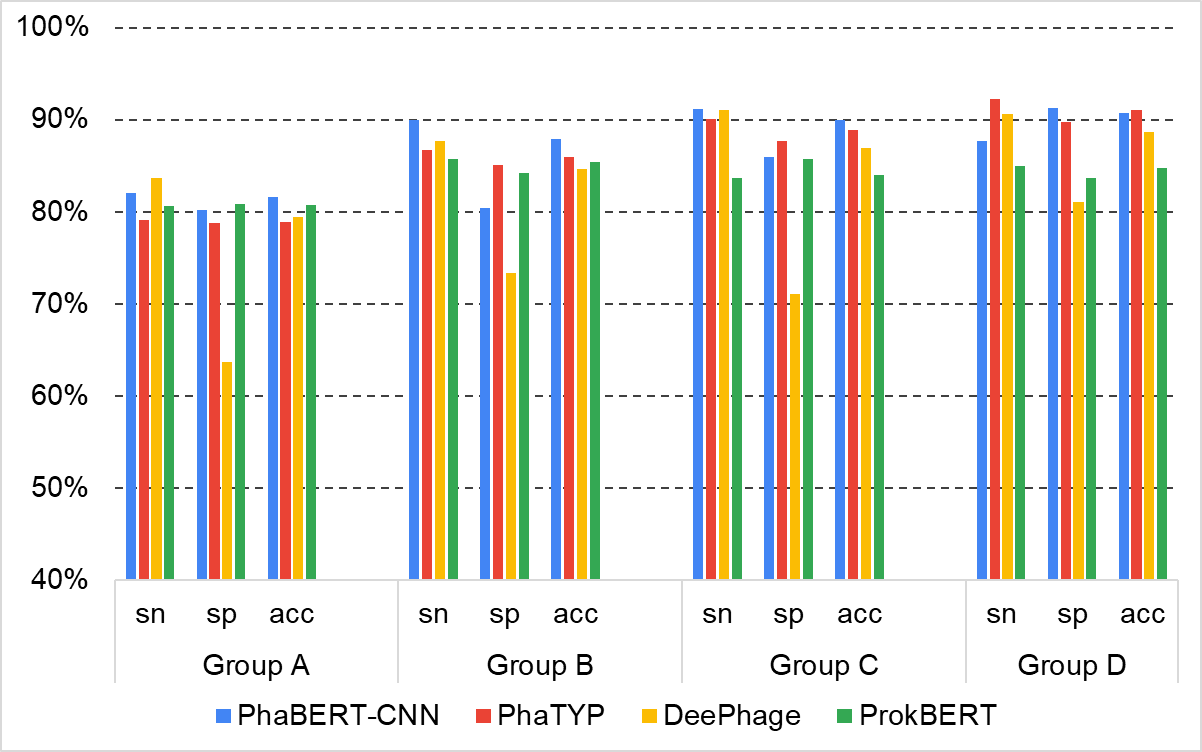
\includegraphics[width=0.85\textwidth]{figures/primary_contig_exp.png}
    \caption{Hiệu suất phân loại của DeePhage, PhaTYP, ProkBERT và PhaBERT trên các nhóm A, B, C, D}
    \label{fig:primary_contig_exp}
\end{figure}

PhaBERT đạt độ chính xác cao nhất trên tất cả bốn nhóm contig, với các giá trị lần lượt là 82,01\%, 87,33\%, 89,90\% và 91,38\%. So với các phương pháp tiên tiến, PhaBERT cải thiện 0,36--3,09\% so với PhaTYP, 2,29--3,94\% so với DeePhage, và 1,33--6,65\% so với ProkBERT. Đặc biệt, mô hình duy trì độ nhạy cao (82,07\%--92,38\%) trong khi đạt độ đặc hiệu ở mức cạnh tranh (81,86\%--87,63\%), cho thấy khả năng phân loại cân bằng giữa hai lớp thực khuẩn. Sự cân bằng này có ý nghĩa thực tiễn quan trọng: độ nhạy cao đảm bảo phát hiện đầy đủ thực khuẩn thể độc lực cho ứng dụng liệu pháp điều trị~\cite{azimi2019phage}, trong khi độ đặc hiệu cao giảm thiểu phân loại sai thực khuẩn thể ôn hòa, vốn có thể mang gen tiềm ẩn không phù hợp cho liệu pháp~\cite{feiner2015new}.

Đáng chú ý, trên Nhóm D (1200--1800 bp), PhaBERT cao hơn PhaTYP với 91,38\% so với 91,02\% về độ chính xác và 92,38\% so với 92,29\% về độ nhạy. PhaTYP vẫn đạt độ đặc hiệu cao hơn ở Nhóm D (89,75\% so với 87,63\%), cho thấy đặc trưng protein mang lại lợi thế trong việc nhận diện phage ôn hòa trên các contig dài chứa đầy đủ các vùng mã hóa protein. Tuy nhiên, PhaBERT đạt hiệu suất tổng thể cao hơn nhờ độ nhạy vượt trội, đồng thời vượt DeePhage 2,29\% và ProkBERT 6,65\% trên nhóm này.

DeePhage~\cite{wu2021deephage} đạt độ chính xác từ 78,07\% đến 89,09\%, cải thiện đều đặn theo độ dài contig nhưng luôn thấp hơn PhaBERT và PhaTYP. Độ đặc hiệu thấp hơn độ nhạy trên tất cả các nhóm (chênh lệch 8--10\%), cho thấy mô hình có xu hướng thiên lệch về phân loại phage độc lực do sử dụng mã hóa one-hot không mang thông tin ngữ cảnh và huấn luyện từ đầu trên tập dữ liệu giới hạn. Tuy nhiên, DeePhage vượt ProkBERT ở Nhóm C (87,37\% so với 84,03\%) và Nhóm D (89,09\% so với 84,73\%), cho thấy kiến trúc CNN vẫn có khả năng cạnh tranh với các mô hình Transformer khi contig đủ dài để chứa các mô-típ chức năng hoàn chỉnh.

ProkBERT~\cite{ligeti2024prokbert} thể hiện hiện tượng bão hòa: độ chính xác đạt cao nhất ở Nhóm B (85,35\%) rồi giảm xuống 84,03\% (Nhóm C) và 84,73\% (Nhóm D), trở thành phương pháp có hiệu suất thấp nhất trên contig dài. Hiện tượng này phản ánh hạn chế của chiến lược mã hóa LCA k-mer chồng lấn, gây rò rỉ thông tin trong quá trình tiền huấn luyện và tạo dư thừa token~\cite{zhou2023dnabert}. Ngược lại, mã hóa BPE~\cite{sennrich2015neural} trong PhaBERT loại bỏ hoàn toàn hiện tượng rò rỉ thông tin đồng thời giảm độ dài chuỗi token khoảng 5 lần, cho phép mô hình khai thác hiệu quả các trình tự dài hơn.

\section{Thảo luận}
\label{sec:thao_luan}

Phần này phân tích các yếu tố đóng góp vào hiệu suất của PhaBERT, đánh giá xu hướng theo độ dài contig và so sánh các chiến lược biểu diễn chuỗi của các phương pháp được đánh giá.

\subsection{Phân tích đóng góp kiến trúc}
\label{sec:kien_truc_contribution}

Hiệu suất vượt trội của PhaBERT trên tất cả bốn nhóm contig xuất phát từ ba yếu tố bổ trợ lẫn nhau. Thứ nhất, PhaBERT hoạt động trực tiếp trên chuỗi DNA thô thông qua mã hóa BPE~\cite{sennrich2015neural}, không phụ thuộc vào công cụ dự đoán gen như Prodigal~\cite{hyatt2010prodigal} mà PhaTYP yêu cầu. Trên các contig ngắn, Prodigal thường không phát hiện được các vùng mã hóa protein hoàn chỉnh do chuỗi quá ngắn để chứa các khung đọc mở đầy đủ~\cite{trimble2012short}, khiến PhaTYP mất đi nguồn thông tin chính; trong khi đó PhaBERT vẫn khai thác được tín hiệu từ trình tự nucleotide thô. Thứ hai, DNABERT-2 đã được tiền huấn luyện trên tập dữ liệu di truyền đa loài quy mô lớn~\cite{zhou2023dnabert}, cho phép mô hình tổng quát hóa tốt hơn so với DeePhage vốn được huấn luyện từ đầu trên tập dữ liệu có kích thước hạn chế---một ưu thế của học chuyển giao đã được chứng minh rộng rãi trong lĩnh vực xử lý ngôn ngữ tự nhiên~\cite{howard2018universal,devlin2019bert}. Thứ ba, kiến trúc MKC với ba nhánh tích chập song song có kích thước cửa sổ 3, 5, 7~\cite{kim2014convolutional} kết hợp với gộp trung bình có mặt nạ cho phép mô hình đồng thời nắm bắt các đặc trưng cục bộ ở nhiều tỷ lệ không gian và tổng hợp thông tin toàn cục, bổ sung hiệu quả cho biểu diễn ngữ cảnh từ bộ mã hóa transformer. Kết quả loại bỏ từng kích thước cửa sổ (Bảng~\ref{tab:ablation_results}) cho thấy các nhánh tích chập có mức đóng góp tương đương nhau và thông tin giữa chúng chồng lấn đáng kể---phù hợp với nhận định của Zhang và Wallace~\cite{zhang2017sensitivity} rằng hiệu suất của mạng tích chập đa cửa sổ ít nhạy cảm với việc lựa chọn kích thước bộ lọc cụ thể, mà phụ thuộc chủ yếu vào việc sử dụng đồng thời nhiều kích thước.

\subsection{Phân tích xu hướng theo độ dài contig}
\label{sec:xu_huong_do_dai}

Kết quả so sánh giữa đường cơ sở DNABERT-2 và PhaBERT (Bảng~\ref{tab:ablation_results}) cho thấy đóng góp của mô-đun MKC tăng dần theo độ dài contig: độ chính xác cải thiện từ 0,49\% ở Nhóm A (từ 81,52\% lên 82,01\%) đến 3,02\% ở Nhóm D (từ 88,36\% lên 91,38\%). Xu hướng này phản ánh rằng khi trình tự dài hơn, các mô-típ chức năng đặc trưng của hệ gen thực khuẩn thể như các vùng điều hòa, các gen liên quan đến chu trình tan và chu trình tiềm tan trở nên hoàn chỉnh hơn, cho phép các bộ lọc tích chập ở nhiều tỷ lệ không gian~\cite{kim2014convolutional} khai thác hiệu quả hơn.

Trên toàn bộ bốn nhóm, PhaBERT là phương pháp duy nhất đạt độ chính xác cao nhất ở tất cả các nhóm và duy trì mức cải thiện đều đặn từ contig ngắn đến contig dài, trong khi các phương pháp còn lại đều thể hiện hạn chế ở một số nhóm nhất định: PhaTYP đạt hiệu suất thấp ở Nhóm A (78,92\%), DeePhage luôn thấp hơn PhaBERT và PhaTYP dù cải thiện đều đặn theo độ dài, và ProkBERT gặp hiện tượng bão hòa từ Nhóm B trở đi khiến hiệu suất giảm xuống thấp nhất trên contig dài.

\subsection{So sánh chiến lược biểu diễn chuỗi}
\label{sec:bieu_dien_chuoi}

Kết quả thực nghiệm cho phép rút ra một số nhận xét về ảnh hưởng của chiến lược biểu diễn chuỗi đến hiệu suất phân loại. Mã hóa BPE~\cite{sennrich2015neural} được sử dụng trong DNABERT-2 và PhaBERT thể hiện ưu thế rõ rệt nhờ ba đặc tính: loại bỏ hiện tượng rò rỉ thông tin giữa các token liền kề, giảm độ dài chuỗi token khoảng 5 lần so với trình tự gốc, và chuyển đổi bài toán mô hình hóa ngôn ngữ có mặt nạ thành bài toán dự đoán đoạn, vốn đã được chứng minh là cải thiện chất lượng học biểu diễn~\cite{raffel2020exploring}. Phương pháp mã hóa dựa trên protein của PhaTYP~\cite{shang2023phatyp} đạt độ đặc hiệu cao nhất trên contig dài (Nhóm D: 89,75\%) nhờ khai thác thông tin ở cấp độ protein, tuy nhiên PhaBERT vẫn tốt hơn về độ chính xác tổng thể (91,38\% so với 91,02\%) nhờ độ nhạy cao hơn. Phương pháp này cũng phụ thuộc vào Prodigal~\cite{hyatt2010prodigal}, công cụ dự đoán gen có hiệu quả giảm đáng kể trên các đoạn DNA ngắn~\cite{trimble2012short}. Mã hóa one-hot trong DeePhage~\cite{wu2021deephage} là chiến lược biểu diễn đơn giản nhất, không mang thông tin ngữ cảnh và không tận dụng tri thức từ tiền huấn luyện, dẫn đến hiệu suất thấp nhất trên contig ngắn; tuy nhiên, kiến trúc CNN cho phép DeePhage cải thiện đều đặn và vượt ProkBERT trên contig dài nhờ khả năng khai thác các mô-típ cục bộ khi trình tự đủ dài. Mã hóa LCA k-mer trong ProkBERT~\cite{ligeti2024prokbert} là phương pháp duy nhất cho thấy hiện tượng bão hòa trên trình tự dài, phản ánh hạn chế cơ bản của việc sử dụng k-mer chồng lấn~\cite{zhou2023dnabert}.

Nhìn chung, kết quả thực nghiệm khẳng định rằng sự kết hợp giữa chiến lược mã hóa hiệu quả (BPE), tiền huấn luyện trên dữ liệu đa dạng (DNABERT-2) và kiến trúc trích xuất đặc trưng chuyên biệt cho tác vụ (MKC) tạo nên lợi thế tổng hợp, cho phép PhaBERT đạt hiệu suất tốt trên phổ độ dài contig phổ biến trong phân tích hệ gen môi trường.

\subsection{Ý nghĩa thực tiễn của cải thiện hiệu suất}
\label{sec:practical_significance}

Trong bối cảnh liệu pháp phage, việc phân loại chính xác lối sống thực khuẩn thể có ý nghĩa an toàn quan trọng. Các hướng dẫn thực hành lâm sàng khuyến nghị ưu tiên sử dụng thực khuẩn thể độc lực cho điều trị, do thực khuẩn thể ôn hòa tiềm ẩn rủi ro biến đổi tiềm tan~\cite{feiner2015new}. Khi phage ôn hòa bị phân loại sai thành độc lực và được sử dụng trong điều trị, chúng có thể tích hợp vào hệ gen vi khuẩn dưới dạng prophage, từ đó chuyển các gen độc lực cho vật chủ thông qua cơ chế chuyển gen ngang~\cite{brussow2004phages}. Các ví dụ điển hình đã được ghi nhận bao gồm độc tố tả (CTXphi), độc tố Shiga (stx1/stx2) và độc tố bạch hầu. Ngược lại, khi phage độc lực bị phân loại sai thành ôn hòa, các ứng viên điều trị tiềm năng sẽ bị loại bỏ, đặc biệt đáng tiếc trong bối cảnh kháng kháng sinh đang là vấn đề y tế toàn cầu nghiêm trọng~\cite{azimi2019phage}.

Ở quy mô dữ liệu hệ gen môi trường hiện đại, tác động của cải thiện hiệu suất được khuếch đại đáng kể. Các cơ sở dữ liệu virus từ hệ gen môi trường như IMG/VR hiện chứa hơn 15 triệu trình tự gen virus. Trên quy mô này, cải thiện 1\% độ chính xác tương đương với việc giảm khoảng 150.000 phân loại sai. Với mức cải thiện 0,36--6,65\% mà PhaBERT-CNN đạt được so với các phương pháp tiên tiến, số lượng contig được phân loại đúng có thể lên đến hàng trăm nghìn trên các tập dữ liệu quy mô lớn.

\section{Kết luận}
\label{sec:ket_luan_c4}

Chương này đã trình bày kết quả đánh giá toàn diện PhaBERT trên bốn nhóm độ dài contig thông qua kiểm định chéo phân tầng 5 phần, bao gồm nghiên cứu loại bỏ thành phần với bảy cấu hình (DNABERT-2, PhaBERT, DNABERT-2-CNN, DNABERT-2-P, PhaBERT-NO-K5, PhaBERT-NO-K3 và PhaBERT-NO-K7), cùng so sánh với ba phương pháp tiên tiến khác. Kết quả nghiên cứu loại bỏ thành phần cho thấy mô-đun MKC cải thiện độ chính xác từ 0,49\% đến 3,02\% so với đường cơ sở DNABERT-2, trong đó mức cải thiện độ đặc hiệu đặc biệt đáng kể (lên đến 8,61\% ở Nhóm A). So sánh các thành phần riêng lẻ cho thấy gộp chú ý (DNABERT-2-P) mang lại lợi thế trên contig ngắn, trong khi CNN đa cửa sổ (DNABERT-2-CNN) phát huy hiệu quả trên contig trung bình và dài; sự kết hợp cả hai nhánh trong PhaBERT mang lại hiệu suất cân bằng và ổn định nhất trên toàn phổ độ dài. Kết quả loại bỏ từng kích thước cửa sổ tích chập cho thấy các nhánh có mức đóng góp tương đương và thông tin chồng lấn đáng kể---lợi ích biên giảm dần khi thêm nhánh, nhưng sự kết hợp đa tỷ lệ vẫn mang lại tính ổn định cao hơn so với từng thành phần riêng lẻ, đặc biệt trên contig dài. Trong so sánh toàn diện với các phương pháp tiên tiến, PhaBERT đạt độ chính xác cao nhất trên tất cả bốn nhóm contig (100--1.800 bp) với khoảng từ 82,01\% đến 91,38\%, cải thiện từ 0,36 đến 6,65\% so với phương pháp tốt nhất tiếp theo. Phân tích cho thấy ba yếu tố chính đóng góp vào hiệu suất này: xử lý trực tiếp trên trình tự DNA thô thông qua mã hóa BPE, học chuyển giao từ mô hình nền tảng tiền huấn luyện trên dữ liệu đa loài, và trích xuất đặc trưng đa tỷ lệ từ mô-đun MKC. Chương tiếp theo tổng kết các đóng góp của nghiên cứu, thảo luận các hạn chế và đề xuất hướng phát triển trong tương lai.